\section{Menus and actions}\label{menus-and-actions}

\subsection{Menus}\label{menus}

Users often use menus to tell a command to the application. It is like
this:

\begin{figure}
\centering
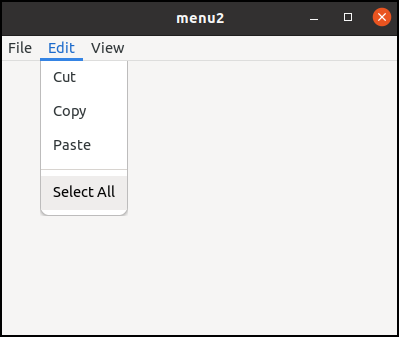
\includegraphics[width=5.985cm,height=5.055cm]{../image/menu.png}
\caption{Menu}
\end{figure}

There are two types of objects.

\begin{itemize}
\tightlist
\item
  ``File'', ``Edit'', ``View'', ``Cut'', ``Copy'', ``Paste'' and
  ``Select All''. They are called ``menu item'' or simply ``item''. When
  the user clicks one of these items, then something will happen.
\item
  Menubar, submenu referenced by ``Edit'' item and two sections. They
  are called ``menu''. Menu is an ordered list of items. They are
  similar to arrays.
\end{itemize}

\begin{figure}
\centering
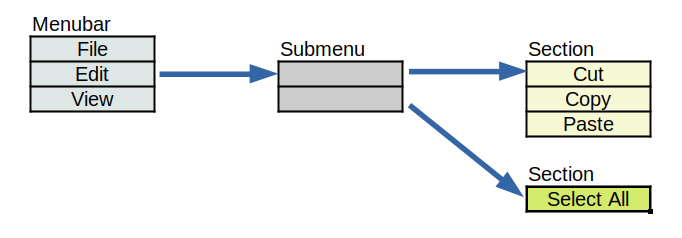
\includegraphics[width=10.23cm,height=3.57cm]{../image/menu_structure.png}
\caption{Menu structure}
\end{figure}

\begin{itemize}
\tightlist
\item
  Menubar is a menu which has three items, which are ``File'', ``Edit''
  and ``View''.
\item
  The menu item labeled ``Edit'' has a link to the submenu which has two
  items. These two items don't have labels. Each item refers to a
  section.
\item
  The first section is a menu which has three items -- ``Cut'', ``Copy''
  and ``Paste''.
\item
  The second section is a menu which has one item -- ``Select All''.
\end{itemize}

Menus can build a complicated structure thanks to the links of menu
items.

\subsection{GMenuModel, GMenu and
GMenuItem}\label{gmenumodel-gmenu-and-gmenuitem}

GMenuModel is an abstract object which represents a menu. GMenu is a
simple implementation of GMenuModel and a child object of GMenuModel.

\begin{lstlisting}
GObject -- GMenuModel -- GMenu
\end{lstlisting}

Because GMenuModel is an abstract object, it isn't instantiatable.
Therefore, it doesn't have any functions to create its instance. If you
want to create a menu, use \passthrough{\lstinline!g\_menu\_new!} to
create a GMenu instance. GMenu inherits all the functions of GMenuModel.

GMenuItem is an object directly derived from GObject. GMenuItem and
Gmenu (or GMenuModel) don't have a parent-child relationship.

\begin{lstlisting}
GObject -- GMenuModel -- GMenu
GObject -- GMenuItem
\end{lstlisting}

GMenuItem has attributes. One of the attributes is label. For example,
there is a menu item which has ``Edit'' label in the first diagram.
``Cut'', ``Copy'', ``Paste'' and ``Select All'' are also the labels of
the menu items. Other attributes will be explained later.

Some menu items have a link to another GMenu. There are two types of
links, submenu and section.

GMenuItem can be inserted, appended or prepended to GMenu. When it is
inserted, all of the attributes and link values are copied and stored in
the menu. The GMenuItem itself is not really inserted. Therefore, after
the insertion, GMenuItem is useless and it should be freed. The same
goes for appending or prepending.

The following code shows how to append GMenuItem to GMenu.

\begin{lstlisting}
GMenu *menu = g_menu_new ();
GMenuItem *menu_item_quit = g_menu_item_new ("Quit", "app.quit");
g_menu_append_item (menu, menu_item_quit);
g_object_unref (menu_item_quit);
\end{lstlisting}

\subsection{Menu and action}\label{menu-and-action}

One of the attributes of menu items is an action. This attribute points
an action object.

There are two action objects, GSimpleAction and GPropertyAction.
GSimpleAction is often used. And it is used with a menu item. Only
GSimpleAction is described in this section.

An action corresponds to a menu item will be activated when the menu
item is clicked. Then the action emits an activate signal.

\begin{enumerate}
\def\labelenumi{\arabic{enumi}.}
\tightlist
\item
  menu item is clicked.
\item
  The corresponding action is activated.
\item
  The action emits a signal.
\item
  The connected handler is invoked.
\end{enumerate}

The following code is an example.

\begin{lstlisting}[language=C]
static void
quit_activated(GSimpleAction *action, GVariant *parameter, gpointer app) { ... ... ...}

GSimpleAction *act_quit = g_simple_action_new ("quit", NULL);
g_action_map_add_action (G_ACTION_MAP (app), G_ACTION (act_quit));
g_signal_connect (act_quit, "activate", G_CALLBACK (quit_activated), app);
GMenuItem *menu_item_quit = g_menu_item_new ("Quit", "app.quit");
\end{lstlisting}

\begin{itemize}
\tightlist
\item
  The variable \passthrough{\lstinline!menu\_item\_quit!} points a menu
  item. It is actually a pointer, but we often say that
  \passthrough{\lstinline!menu\_item\_quit!} \emph{is} a menu item. It
  has a label ``Quit'' and is connected to an action ``app.quit''.
  ``app'' is a prefix and ``quit'' is the name of the action. The prefix
  ``app'' means that the action belongs to the GtkApplication instance.
\item
  \passthrough{\lstinline!act\_quit!} is an action. It has a name
  ``quit''. The function
  \passthrough{\lstinline!g\_simple\_action\_new!} creates a stateless
  action. So, \passthrough{\lstinline!act\_quit!} is stateless. The
  meaning of stateless will be explained later. The argument
  \passthrough{\lstinline!NULL!} means that the action doesn't have an
  parameter. Most of the actions are stateless and have no parameter.
\item
  The action \passthrough{\lstinline!act\_quit!} is added to the
  GtkApplication instance with
  \passthrough{\lstinline!g\_action\_map\_add\_action!}. So, the
  action's scope is application. The prefix of
  \passthrough{\lstinline!app.quit!} indicates the scope.
\item
  ``activate'' signal of the action is connected to the handler
  \passthrough{\lstinline!quit\_activated!}.
\end{itemize}

If the menu is clicked, the corresponding action ``quit'' will be
activated and emits an ``activate'' signal. Then, the handler
\passthrough{\lstinline!quit\_activated!} is called.

\subsection{Menu bar}\label{menu-bar}

A menu bar and menus are traditional. Menu buttons are often used
instead of a menu bar lately, but the old style is still used widely.

Applications have only one menu bar. If an application has two or more
windows which have menu bars, the menu bars are exactly the same.
Because every window refers to the same menubar instance in the
application.

An application's menu bar is usually unchanged once it is set. So, it is
appropriate to set it in the ``startup'' handler. Because the handler is
called only once in the primary application instance.

I think it is good for readers to clarify how applications behave.

\begin{itemize}
\tightlist
\item
  When an application runs for the first time, the instance is called
  primary.
\item
  The primary instance registers itself to the system. If it succeeds,
  it emits ``startup'' signal.
\item
  When the instance is activated, an ``activate'' or ``open'' signal is
  emitted.
\item
  If the application is run for the second time or later and there
  exists a primary instance, the instance is called a remote instance.
\item
  A remote instance doesn't emit ``startup'' signal.
\item
  If it tries to emit an ``activate'' or ``open'' signal, the signals
  are not emitted on the remote instance but primary instance.
\item
  The remote instance quits.
\end{itemize}

Therefore, an ``activate'' or ``open'' handler can be called twice or
more. On the other hand, a ``startup'' handler is called once. So, the
menubar should be set in the ``startup'' handler.

\begin{lstlisting}[language=C]
static void
app_startup (GApplication *app) {
... ... ...
  gtk_application_set_menubar (GTK_APPLICATION (app), G_MENU_MODEL (menubar));
... ... ...
}
\end{lstlisting}

\subsection{Simple example}\label{simple-example}

The following is a simple example of menus and actions. The source file
\passthrough{\lstinline!menu1.c!} is located at src/menu directory.

\begin{lstlisting}[language=C, numbers=left]
#include <gtk/gtk.h>

static void
quit_activated(GSimpleAction *action, GVariant *parameter, GApplication *application) {
  g_application_quit (application);
}

static void
app_activate (GApplication *application) {
  GtkApplication *app = GTK_APPLICATION (application);
  GtkWidget *win = gtk_application_window_new (app);
  gtk_window_set_title (GTK_WINDOW (win), "menu1");
  gtk_window_set_default_size (GTK_WINDOW (win), 400, 300);

  gtk_application_window_set_show_menubar (GTK_APPLICATION_WINDOW (win), TRUE);
  gtk_window_present (GTK_WINDOW (win));
}

static void
app_startup (GApplication *application) {
  GtkApplication *app = GTK_APPLICATION (application);

  GSimpleAction *act_quit = g_simple_action_new ("quit", NULL);
  g_action_map_add_action (G_ACTION_MAP (app), G_ACTION (act_quit));
  g_signal_connect (act_quit, "activate", G_CALLBACK (quit_activated), application);

  GMenu *menubar = g_menu_new ();
  GMenuItem *menu_item_menu = g_menu_item_new ("Menu", NULL);
  GMenu *menu = g_menu_new ();
  GMenuItem *menu_item_quit = g_menu_item_new ("Quit", "app.quit");
  g_menu_append_item (menu, menu_item_quit);
  g_object_unref (menu_item_quit);
  g_menu_item_set_submenu (menu_item_menu, G_MENU_MODEL (menu));
  g_object_unref (menu);
  g_menu_append_item (menubar, menu_item_menu);
  g_object_unref (menu_item_menu);

  gtk_application_set_menubar (GTK_APPLICATION (app), G_MENU_MODEL (menubar));
}

#define APPLICATION_ID "com.github.ToshioCP.menu1"

int
main (int argc, char **argv) {
  GtkApplication *app;
  int stat;

  app = gtk_application_new (APPLICATION_ID, G_APPLICATION_DEFAULT_FLAGS);
  g_signal_connect (app, "startup", G_CALLBACK (app_startup), NULL);
  g_signal_connect (app, "activate", G_CALLBACK (app_activate), NULL);

  stat =g_application_run (G_APPLICATION (app), argc, argv);
  g_object_unref (app);
  return stat;
}
\end{lstlisting}

\begin{itemize}
\tightlist
\item
  3-6: \passthrough{\lstinline!quit\_activated!} is a handler of the
  ``activate'' signal on the action \passthrough{\lstinline!act\_quit!}.
  Handlers of the ``activate'' signal have three parameters.

  \begin{enumerate}
  \def\labelenumi{\arabic{enumi}.}
  \tightlist
  \item
    The action instance on which the signal is emitted.
  \item
    Parameter. In this example it is \passthrough{\lstinline!NULL!}
    because the second argument of
    \passthrough{\lstinline!g\_simple\_action\_new!} (line 23) is
    \passthrough{\lstinline!NULL!}. You don' t need to care about it.
  \item
    User data. It is the fourth parameter in the
    \passthrough{\lstinline!g\_signal\_connect!} (line 25) that connects
    the action and the handler.
  \end{enumerate}
\item
  5: The function \passthrough{\lstinline!g\_application\_quit!}
  immediately quits the application.
\item
  8-17: \passthrough{\lstinline!app\_activate!} is an ``activate''
  signal handler on the application.
\item
  11-13: Creates a GtkApplicationWindow \passthrough{\lstinline!win!}.
  And sets the title and the default size.
\item
  15: Sets GtkApplicationWindow to show the menubar.
\item
  16: Shows the window.
\item
  19-38: \passthrough{\lstinline!app\_startup!} is a ``startup'' signal
  handler on the application.
\item
  23: Creates GSimpleAction \passthrough{\lstinline!act\_quit!}. It is
  stateless. The first argument of
  \passthrough{\lstinline!g\_simple\_action\_new!} is a name of the
  action and the second argument is a parameter. If you don't need the
  parameter, pass \passthrough{\lstinline!NULL!}. Therefore,
  \passthrough{\lstinline!act\_quit!} has a name ``quit'' and no
  parameter.
\item
  24: Adds the action to GtkApplication \passthrough{\lstinline!app!}.
  GtkApplication implements an interface GActionMap and GActionGroup.
  GtkApplication (GActionMap) can have a group of actions and the
  actions are added with the function
  \passthrough{\lstinline!g\_action\_map\_add\_action!}. This function
  is described in
  \href{https://docs.gtk.org/gio/method.ActionMap.add_action.html}{Gio
  API Reference -- g\_action\_map\_add\_action}. Because this action
  belongs to GtkApplication, its scope is ``app'' and it is referred
  with ``app.quit'' if the prefix (scope) is necessary.
\item
  25: Connects ``activate'' signal of the action and the handler
  \passthrough{\lstinline!quit\_activated!}.
\item
  27-30: Creates GMenu and GMenuItem instances.
  \passthrough{\lstinline!menubar!} and \passthrough{\lstinline!menu!}
  are GMenu. \passthrough{\lstinline!menu\_item\_menu!} and
  \passthrough{\lstinline!menu\_item\_quit!} are GMenuItem.
  \passthrough{\lstinline!menu\_item\_menu!} has a label ``Menu'' and no
  action. \passthrough{\lstinline!menu\_item\_quit!} has a label
  ``Quit'' and an action ``app.quit''.
\item
  31-32: Appends \passthrough{\lstinline!menu\_item\_quit!} to
  \passthrough{\lstinline!menu!}. As I mentioned before, all the
  attributes and links are copied and used to form a new item in
  \passthrough{\lstinline!menu!}. Therefore after the addition,
  \passthrough{\lstinline!menu\_item\_quit!} is no longer needed. It is
  freed by \passthrough{\lstinline!g\_object\_unref!}.
\item
  33-34: Sets the submenu link in
  \passthrough{\lstinline!menu\_item\_menu!} to point
  \passthrough{\lstinline!menu!}. Then, \passthrough{\lstinline!menu!}
  is no more useful and it is freed.
\item
  35-36: Appends \passthrough{\lstinline!menu\_item\_menu!} to
  \passthrough{\lstinline!menubar!}. Then frees
  \passthrough{\lstinline!menu\_item\_menu!}. GMenu and GMenuItem are
  built and finally connected to the variable
  \passthrough{\lstinline!menubar!}. The structure of the menu is shown
  in the diagram below.
\item
  38: The menubar is inserted to the application.
\end{itemize}

\begin{figure}
\centering
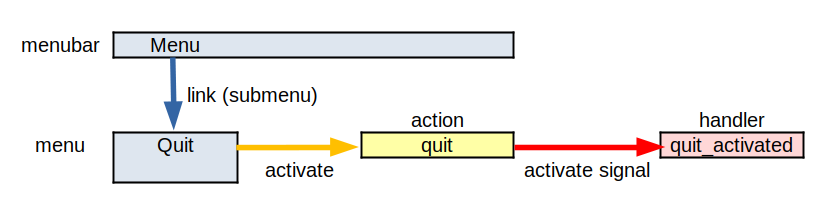
\includegraphics[width=12.555cm,height=3.285cm]{../image/menu1.png}
\caption{menu and action}
\end{figure}

\subsection{Compiling}\label{compiling}

Change your current directory to \passthrough{\lstinline!src/menu!}. Use
comp to compile \passthrough{\lstinline!menu1.c!}.

\begin{lstlisting}
$ comp menu1
$ ./a.out
\end{lstlisting}

Then, a window appears. Click on ``Menu'' on the menubar, then a menu
appears. Click on ``Quit'' menu, then the application quits.

\begin{figure}
\centering
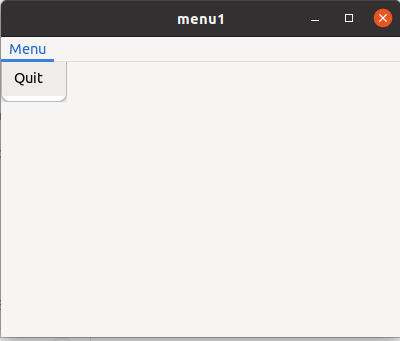
\includegraphics[width=6cm,height=5.115cm]{../image/menu1_screenshot.png}
\caption{Screenshot of menu1}
\end{figure}

\subsection{Primary and remote application
instances}\label{primary-and-remote-application-instances}

Let's try running the application twice. Use
\passthrough{\lstinline!\&!} in your shell command line, then the
application runs concurrently.

\begin{lstlisting}
$ ./a.out &
[1] 70969
$ ./a.out
$ 
\end{lstlisting}

Then, two windows appear.

\begin{itemize}
\tightlist
\item
  The first \passthrough{\lstinline!./a.out!} calls the application and
  a primary instance is created. It calls ``startup'' and ``activate''
  handlers and shows a window.
\item
  The second\passthrough{\lstinline!./a.out!} calls the the application
  again and the created instance is a remote one. It doesn't emit
  ``startup'' signal. And it activates the application but the
  ``activate'' signal is emitted on the primary instance. The remote
  instance quits.
\item
  The primary instance called ``activate'' handler. The handler creates
  a new window. It adds a menu bar to the window with
  \passthrough{\lstinline!gtk\_application\_window\_set\_show\_menubar!}
  function.
\end{itemize}

Both the windows have menu bars. And they are exactly the same. The two
windows belong to the primary instance.

If you click on the ``Quit'' menu, the application (the primary
instance) quits.

\begin{figure}
\centering
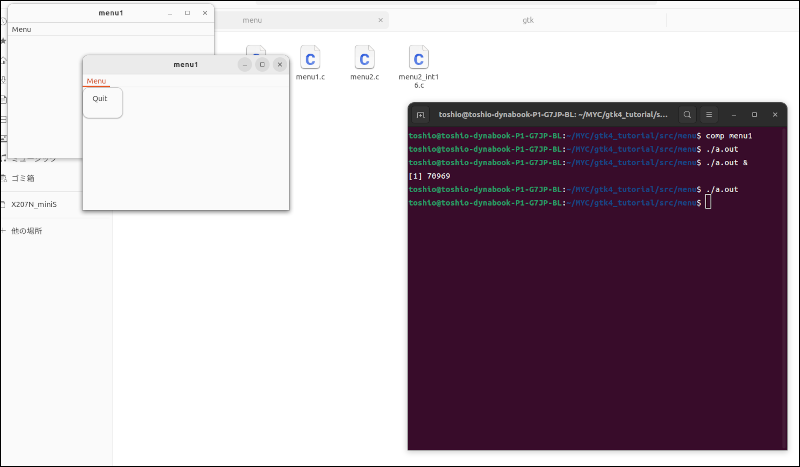
\includegraphics[width=12cm,height=7cm]{../image/menu1_two_windows.png}
\caption{menu1 -- two windows}
\end{figure}

The second execution makes a new window. However, it depends on the
``activate'' handler. If you create your window in the startup handler
and the activate handler just presents the window, no new window is
created at the second execution. For example, tfe (text file editor)
doesn't create a second window. It just creates a new notebook page.
Because its activate handler doesn't create any window but just creates
a new notebook page.

Second or more executions often happen on the desktop applications. If
you double-click the icon twice or more, the application is run multiple
times. Therefore, you need to think about your startup and activate
(open) handler carefully.
